\documentclass{article} % book, report, letter
\usepackage{geometry}
\usepackage{ctex} %中文
\usepackage{graphicx}
\usepackage{listings}
\usepackage[usenames,dvipsnames]{xcolor}
\geometry{a4paper,a4paper,left=2cm,right=2cm,top=1cm,bottom=1cm}
\lstset{language=C++}
\title{\LARGE 网络编程大作业东南大学网络拓扑自动构造}
\author{\Large 71118225 赵君亮}
\date{\today}
\begin{document}
    \maketitle %输出标题
    \section{\LARGE 网络拓扑构造原理}
    \par 网络拓扑结构是指用传输媒体互连各种设备的物理布局
    (将参与LAN工作的各种设备用媒体互连在一起有多种方法,
    但是实际上只有几种方式能适合LAN的工作)。
    要构造网络拓扑图,可以通过ping出网络结构种的活跃节点,并且通过tracert追踪指令
    去追踪该活跃节点,通过多次追踪,找到不同路径,确定网络拓扑种的主干节点。
    \section{\LARGE 东南大学校园网结构}
    \par 为了实现本次网络拓扑图的自动构造,首先要去探究实验网络环境,对于东南大学,是校
    园网的一种,它需要划分不同的子网来提供给学生和老师使用 。
    \par 东南大学依据教学区、生活区以及专业楼等不同场所划分不同的子网结构,下图是通过信息
    网获取的官方东南大学拓扑结构。\\
    \\
    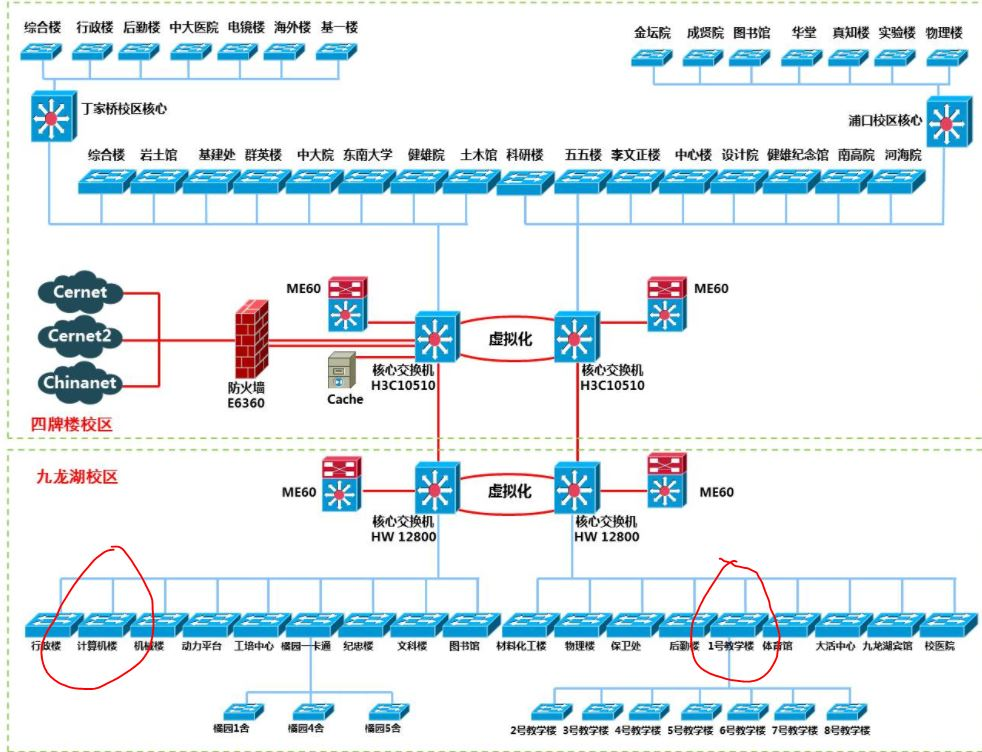
\includegraphics[scale=0.5]{pic/东南大学网络拓扑图.JPG}
    \\
    \\
    \\
    \par 从东南大学的网络拓扑结构,我们很明显可以看出来,其各个子网是由交换机控制的,
    并且该拓扑结构相对比较简单,仅仅是交换机的二层结构,对于网络拓扑结构
    的构建大大减少了工作难度。
    校园内部网络是有防火墙阻隔,防止外网入侵。在这个子网拓扑图中,本次实验主要选择教学楼
    宿舍区以及计算机楼这三个地区作为锚点,进行实验,分析出东南大学传输的主干交换机IP。
    \\
    \par 分析了东南大学的网络拓扑结构,接下来需要了解的是各个子网的IP分配。通过查询东南
    大学信息化中心,可以获得官方给定IP地址。信息来源:https://nic.seu.edu.cn/wlgl/xnIPgl.htm
    
    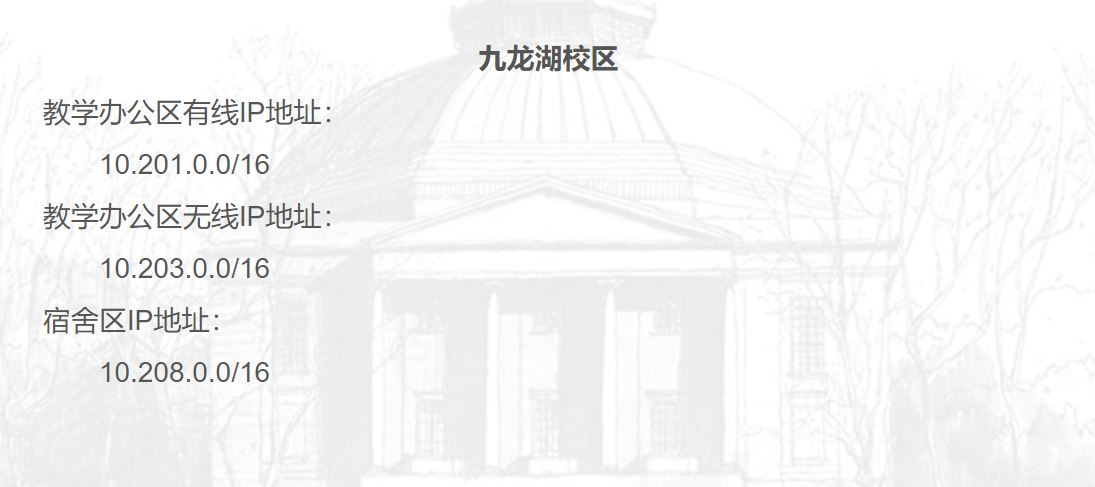
\includegraphics[scale=0.5]{pic/九龙湖ip地址分配.JPG}
    \\
    \par 通过九龙湖校区IP分配,可以很明显得出,东南大学划分的子网掩码是16位。这里采用
    宿舍区10.208.0.0/16 以及 10.203.0.0/16 两个子网进行互ping实验,并且找出其中的
    主干节点,即可以获取东南大学交换机的固定IP地址。
    \par 由于要能ping通,必须处于一个子网下才可以转发,所以可以推测东南大学交换机
    的固定地址存在10.208开头或者10.203开头。有了这些想法和前提条件,可以开始设计实验。
    \section{\LARGE 实验条件说明}
        \subsection{\Large 工具选用}
        \par 在本次实验中,由于需要进行大量数据数据处理和拓扑图的构造,实现较为方便的
        python语言进行编程。对于网络拓扑结构图的构建,采用了图形数据库neo4j进行保存
        存储拓扑图。neo4j是一个比较常用的知识图谱数据库,可以方便的构造出有向图。
        \subsection{\Large 环境说明}
        \par 本次编程是在Windows10的环境下,并且连接了东南大学的校园网的条件下实现的。
        系统环境需要存在ping指令以及tracert指令。
        \subsection{\Large 实验锚点IP选定}
        \par 这里选定了:
        \par 教一 10.19.0.0/16 
        \par 计算机楼以及除了教一以外的其他教学楼 10.203.0.0/16
        \par 宿舍区 10.208.0.0/16
        \par 上述三个为锚点选中。为什么是这样的呢。首先,从日常的校园网使用,不难发现
        教一、宿舍楼以及计算机楼的三个地方的wifi命名是不不同的。此外,通过我的实际测验
        发现,当我迁移位置时,比如从教一到计算机楼的时候,ip地址发生了改变,而且需要重新
        验证连接。但是当我从教二、教四到计算机楼的时候,ip地址是不变的,连接也是会自动连
        不需要验证的。宿舍楼同理,所以这里可以推测学校的这三个位置分属三个子网,
        分别从每个子网取出几个锚点,可以更好的进行主干IP的提取。
    \section{\LARGE 实验设计与实现}
        \subsection{\Large 通过ping获取网络结构的在线活跃点}
        \par 首先对于东南大学的校园网而言是一个局域网,各个子网都是由交换机控制的,之间
        是可以相互转发的。所以针对不同子网而言原理上是可以ping通的。但是由于并不完全处于
        一个子网下,ping会有一定的延迟,相较于广域网的延迟而言,这种延迟对本实验并不会产生
        太大的影响。此外还有一个因素也会影响本实验的效率,那便是访问的活跃节点很多事个人主机
        存在着防火墙,有时候并不能ping通,会造成长时间的延迟无反馈。这里就涉及到一个等待
        时间的问题。\\
        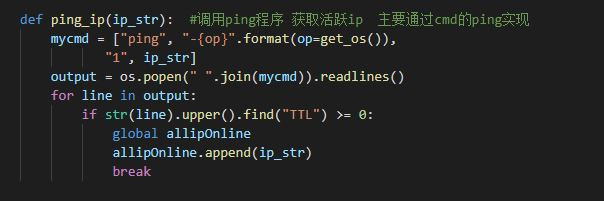
\includegraphics[scale=0.7]{pic/ping代码1.JPG}
        \par 在上述的代码种,首先是先确定了本机的操作系统,方便去调用系统的ping指令
        并且在ping指令种设置了TTL作为是否ping成功的判定依据。如果成功则将该活跃节点保存
        用于后续的节点追踪。
        \par 第二个问题是要解决ping不同的情况,因为其实并非一个子网下的所有动态IP都是ping
        得通的,所以这里是不可以用手动去cmd上进行ping指令的。这里需要写一个脚本去遍历所有
        的动态子IP。举个例子,比如我在教学楼,然后需要ping通宿舍楼的IP,那么这里的话就要ping
        10.208.0.0/16子网下的所有IP,10.208.0.0-10.208.255.255。
        \par 第三个问题是在第二个问题的基础上的,作为cmd的ping指令,其实尝试过
        都可以轻易发现,每个ping指令都是需要很长时间的检查的,ping一个地址,
        约为3-5s反馈结束。所以作为几百上千个的ping,这里就需要调用的一个多线程的操作。
        \\
        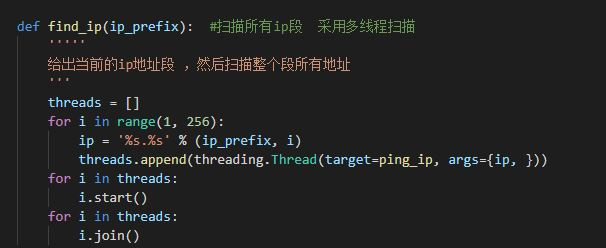
\includegraphics[scale=0.7]{pic/ping代码2.JPG}
        \par 由于不同代码段的对称性,比如10.208.5.0/8 与 10.208.6.0/8路径是相似的
        所以,对于问题二这里可以有一个比较好的修正方案。除了多线程,对于代码段的选取也可以不用
        全选。比如可以从10.208.0.0/8-10.208.40.0/8。然后再在高位代码段选取一段,比如
        10.208.128.0/8-10.208.192.0/8。这样就解决了ping大量IP的时间运行问题了。
        \par 如下图所示,是一个从教一ping宿舍10.208.192.0/8-10.208.193.0/8IP段的实验结果\\
        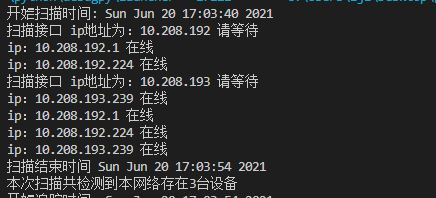
\includegraphics[scale=1.0]{pic/ping结果1.JPG}
        
        \subsection{\Large 通过tracert追踪活跃ip}
        \par 在上述过程完成了活跃节点的获取,并将其保存。接下来就是要对这一列的活跃节点进行
        追踪来获取主干静态IP。首先是要了解与tracert相关的原理和指令。
        \par tracert是一个windows系统的IP追踪指令(linux是traceroute,其多了可以自主选定
        源节点的功能,tracert只支持IPV6的源节点选中,IPV4不支持),tracert具有很多的功能
        \par 如下图所示是tracert一些常用的参数\\
        \\
        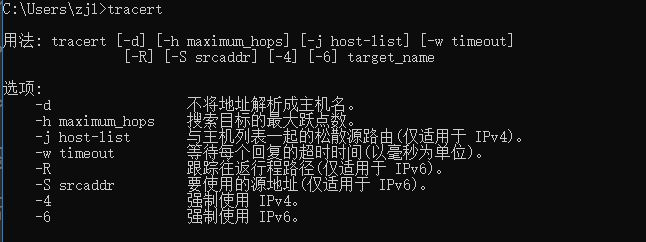
\includegraphics[scale=0.8]{pic/tracert代码1.JPG}
        \par tracert指令可以通过途径各个静态IP追踪到目标IP,并把路径IP显示出来。并且它还具有
        解析主机名的功能。这里有一个值得一提的问题。解析主机名虽然作为一个不错的功能,但是
        在本次实验中探索的是路径,并不需要解析主机名,并且解析主机名要消耗大量的时间,所以在本次实验中,需要在指令
        中加入-d的参数来取消解析主机名这一个操作,来提高运行的效率。
        \par 在进行实验前,这里做了一个小测验来探究tracert的功能,使用tracert探究从本机IP
        到ping通百度IP走过的所有IP节点。\\
        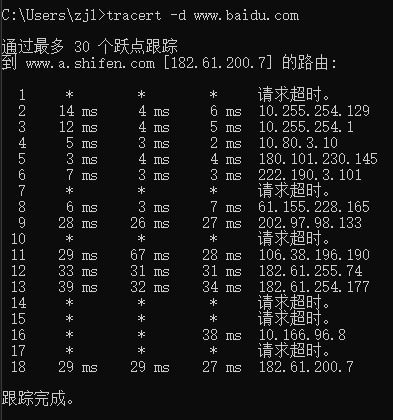
\includegraphics[scale=0.6]{pic/教一追踪百度.JPG}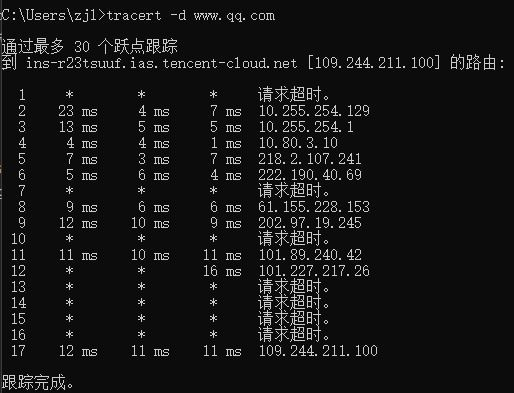
\includegraphics[scale=0.6]{pic/教一追踪qq.JPG}
        \par 在上图可以很清晰的看见一个从本机IP到百度IP的过程。当然中间可能也是会遇到一些
        请求超时的节点,这些节点其实是存在防火墙或者反馈时间过长,导致获取不到该节点IP。
        对于上述问题,大多出现在广域网的路径追踪中。而本次实验,作为局域网,并不会出现中间访问断点的问题。
        \par 另外,从上述对tracert的简单测试,左边是追踪百度网址,右边是追踪qq网址
        很明显可以看出来,追踪的前三项是相同的,这里可以作一个大胆的推测,10.255.254.129   
        10.255.254.1   10.80.3.10这三个IP地址都是学校的主干静态IP,也就是我们需要构造的拓扑图节点
        \subsection{\Large 选取多个网络节点作为锚点重复追踪}
        \par 完成了简单的测试之后,接下来需要在校园网内进行大量追踪实验。
        \par 这里分为从宿舍楼到教一、从宿舍楼到计算机楼、从教一到宿舍楼、从计算机楼到宿舍楼、以及从
        教一到计算机楼的追踪,五个部分的追踪。前面讲述过锚点选用的原因,这里不再赘述。为了
        找到校园网的主干拓扑,必须采用不同子网间的互相追踪才可以获取转发的主干节点。
        \par 对于追踪这部分的程序实现,因为有大量的IP地址需要追踪,所以同样要采用多线程的
        tracert指令运行,并且要带上-d参数,取消目标IP的主机解析。
        \par 追踪代码多线程实现如下图所示\\
        \\
        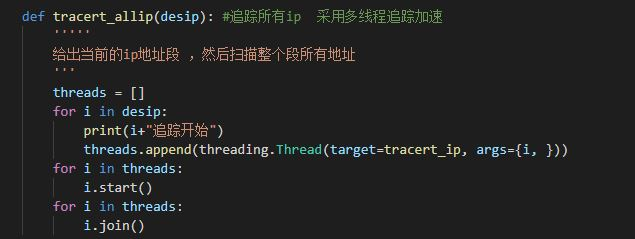
\includegraphics[scale=0.7]{pic/追踪代码1.JPG}\\
        \\
         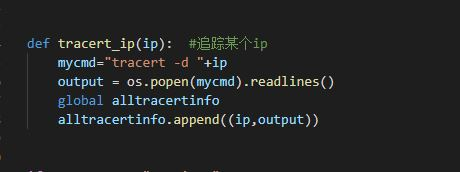
\includegraphics[scale=0.7]{pic/追踪代码2.JPG}
        \subsection{\Large 通过大量追踪数据,找到其中的主干转发节点}
        \par 通过一系列的追踪,程序运行效果如下图所示。\\
        \\
        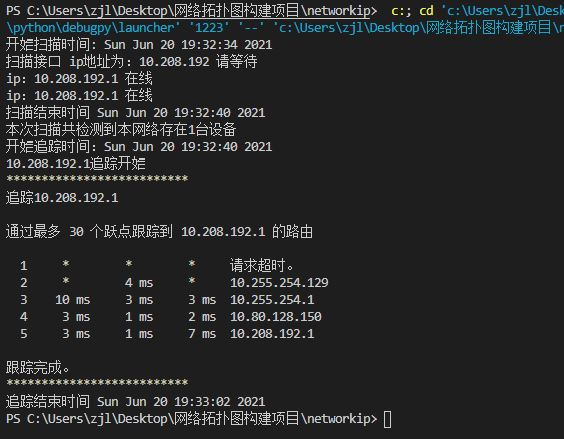
\includegraphics[scale=0.8]{pic/追踪结果1.JPG}
        \par 由图可见,追踪10.208.192.1,经过10.255.254.129  10.255.254.1  10.80.128.150 最后到
        10.208.192.1。这一系列的追踪可以构造出一个图,获得一个路线。
        该路线保存为一个python中的数据结果,map序列。并且通过该序列,判定出非叶子节点
        作为主干节点。如下图所示:\\
        \\
        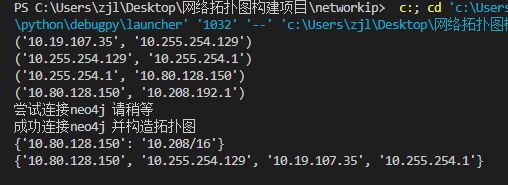
\includegraphics[scale=0.8]{pic/追踪结果2.JPG}
        \par 上图用('10.19.107.35', '10.255.254.129')表示这两个IP之间互相连接转发
        并且通过遍历所有的map数据,得到叶子节点,去除叶子节点,留下主干节点。
        最后获得的主干节点为{'10.80.128.150', '10.255.254.129', '10.19.107.35', '10.255.254.1'}
        \subsection{\Large 利用neo4j数据库构造拓扑图}
        \par 完成了主干节点的提取后,最后一步是构造拓扑图。这里采用的是neo4j的数据库来构造
        网络拓扑图,首先把主干节点都写入,然后将有连接的两个主干节点互相连接起来。
        而由于叶子节点的众多,所以这里直接把叶子节点表示为一个掩码的形式,作为IP集合。比如这里
        的叶子节点都是10.208.0.0/16的IP集合。
        \\
        \par 下图是NEO4J数据库的使用\\
        \\
        \\
        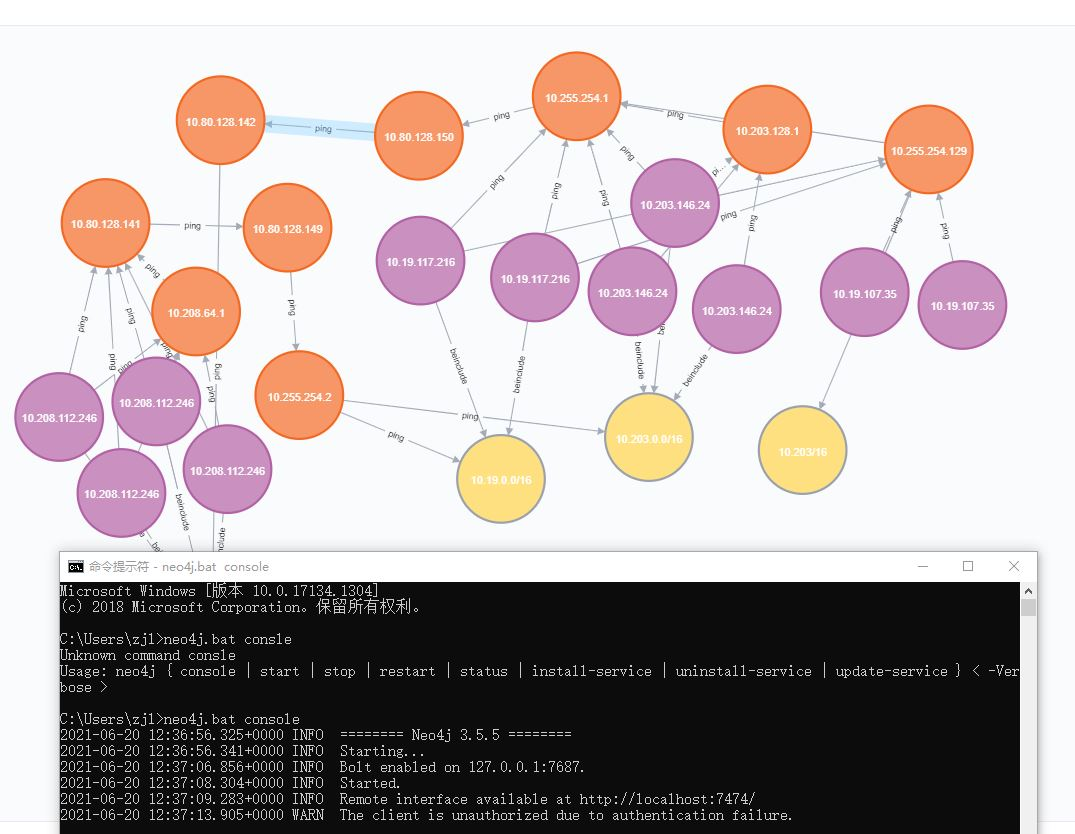
\includegraphics[scale=0.5]{pic/neo4j数据库.JPG}
        \\
        \\
        \\
        \\
        \\
        \\
        \\
        \\
        \\
        \\
        \\
        \\
        \par 下图是构造的结果\\
        \\
        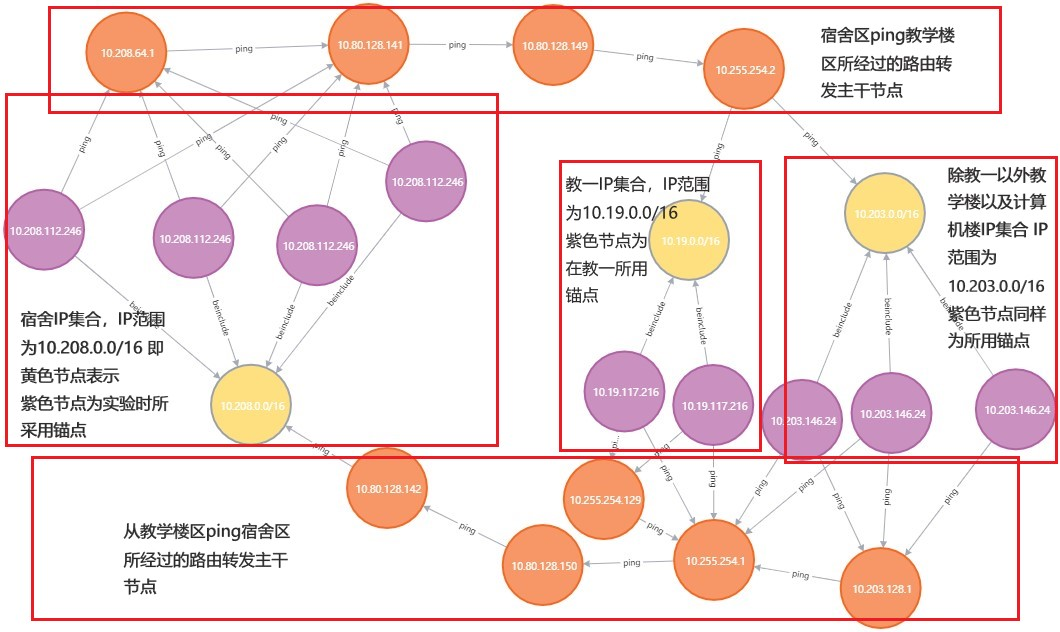
\includegraphics[scale=0.6]{pic/东南大学网络拓扑图说明.jpg}
        \par 通过上图,可以很明显看出来,橙色节点为交换机静态IP,即为主干节点。紫色节点是我本机
        IP,也就是选定的锚点。黄色节点是一个子网的集合IP,紫色节点自然也属于这部分集合。
    \section{\LARGE 实验结果分析与拓展延申}
    \par 现在回过头,取看刚刚在广域网进行的tracert指令。可以发现一些有趣的事情,
    根据百度网址的追踪结果,在校园网拓扑图中标记出现过的节点,如下面右图蓝色部分标注部分\\
    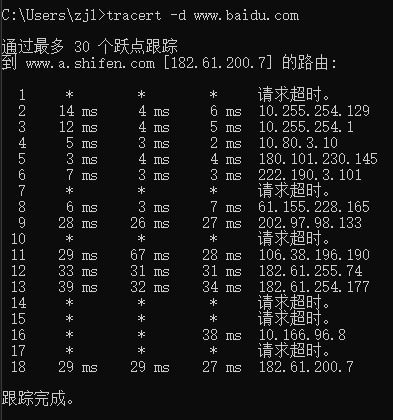
\includegraphics[scale=0.5]{pic/教一追踪百度.JPG} 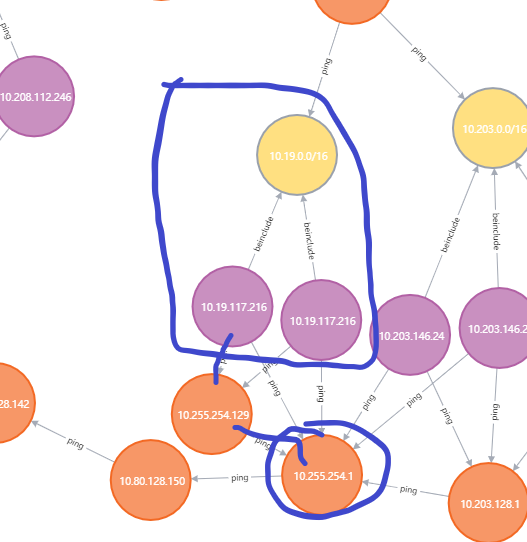
\includegraphics[scale=0.7]{pic/东南大学网络拓扑图.png}
    \par 可以很明显发现,节点追踪到10.255.254.1 后面就是通过10.80.3.10对外转发。以及转发到宿舍网也是经过该节点,
    说明10.255.254.1是东南大学九龙湖教学区对外交换的跟节点。而10.80.3.10很可能是对外转发的IP节点
    为了验证这一个想法,下列继续进行宿舍区对百度进行追踪
    \\
    \\
    \\
    \par 同样可以可以对宿舍追踪百度进行标记,如下图所示\\
    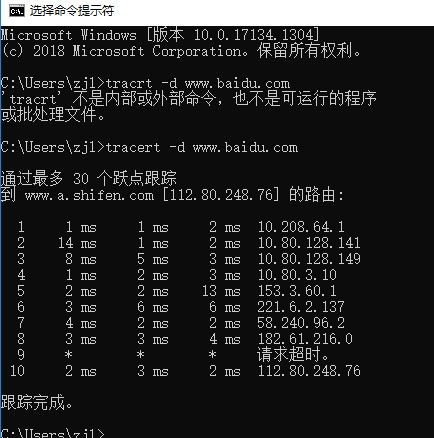
\includegraphics[scale=0.5]{pic/追踪百度.JPG} 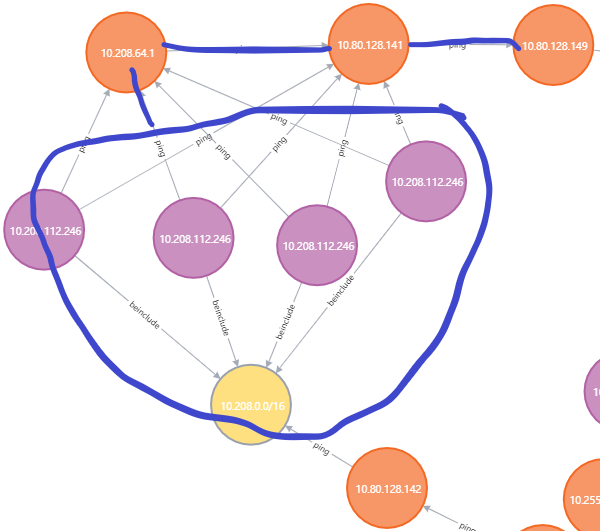
\includegraphics[scale=0.7]{pic/宿舍东南大学网络拓扑图.png}
    \par 对比教一追踪百度网址IP和宿舍区追踪百度网址IP,可以明显该处也是通过10.80.3.10对外转发
    所以这里可以推断,10.80.3.10是整个东南大学九龙湖校区对外转发的IP节点。当然了在内部转发,是不用不到该节点的
    所以在该拓扑图上也就看不见这个节点。
    \section{\LARGE 总结与收获}
    \par 本次实验可以说比较成功,完整的构造了东南大学九龙湖校区的一个网络拓扑结构。通过该图
    可以很容易的了解校园网的结构。
    \par 整个实验流程为:原理了解->官方网络结构分析->构造设计->编写代码->运行代码->收集数据
    ->处理数据->构造网路拓扑图。
    \par 不论是从工具的选择还是实验的设计,该实验都做得比较完善。当然该实验仅仅只是构造了东南大学
    的校园网,并没有对广域网进行一个构建,在后续的学习生活中,可以对其进行一个更好的改进,可以尝试
    去测试广域网的拓扑结构。
    \par 通过该实验,我学习了很多,学会了各个子网之间的转发原理,了解了一个网络拓扑结构是怎样构建的
    以及这样的一个网络结构是如何工作的。更好的去理解了何为IP地址,何为动态IP地址,何为静态IP地址。
    也掌握了ping工具和tracert的使用。
    \par 此外通过整个实验流程的设计和实现,提高了我动手操作的实践能力,以及项目的实现管理能力。

\end{document}